% Regression predictions input and phys.
\begin{figure}[hp]
    \begin{subfigure}[b]{\linewidth}
    	\centering
        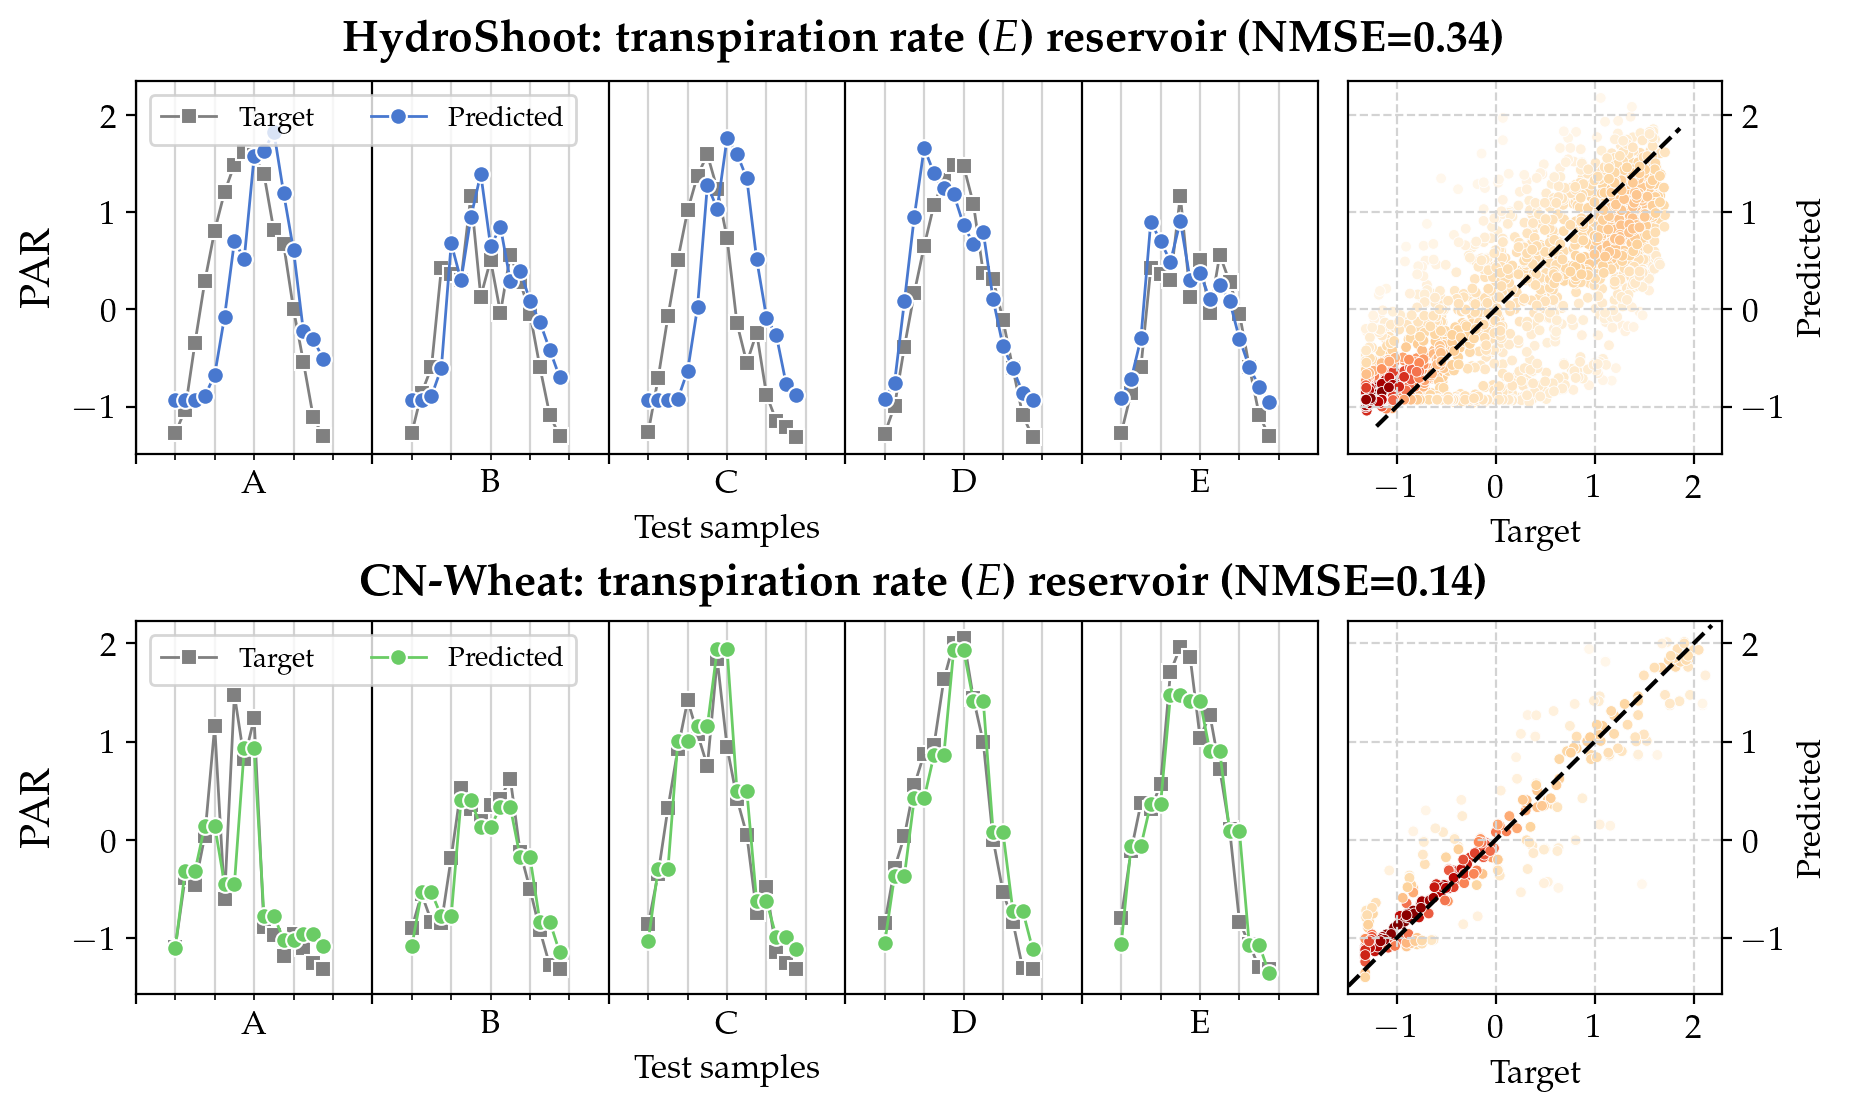
\includegraphics[width=\linewidth,keepaspectratio]{img/regression_res_prediction__input_PARi__state__Tr.png}
        \caption{Time series prediction of input PAR.}
    	\label{fig:predictions-input}
	\end{subfigure}
	\vskip\baselineskip
	\begin{subfigure}[b]{\linewidth}
	    \centering
        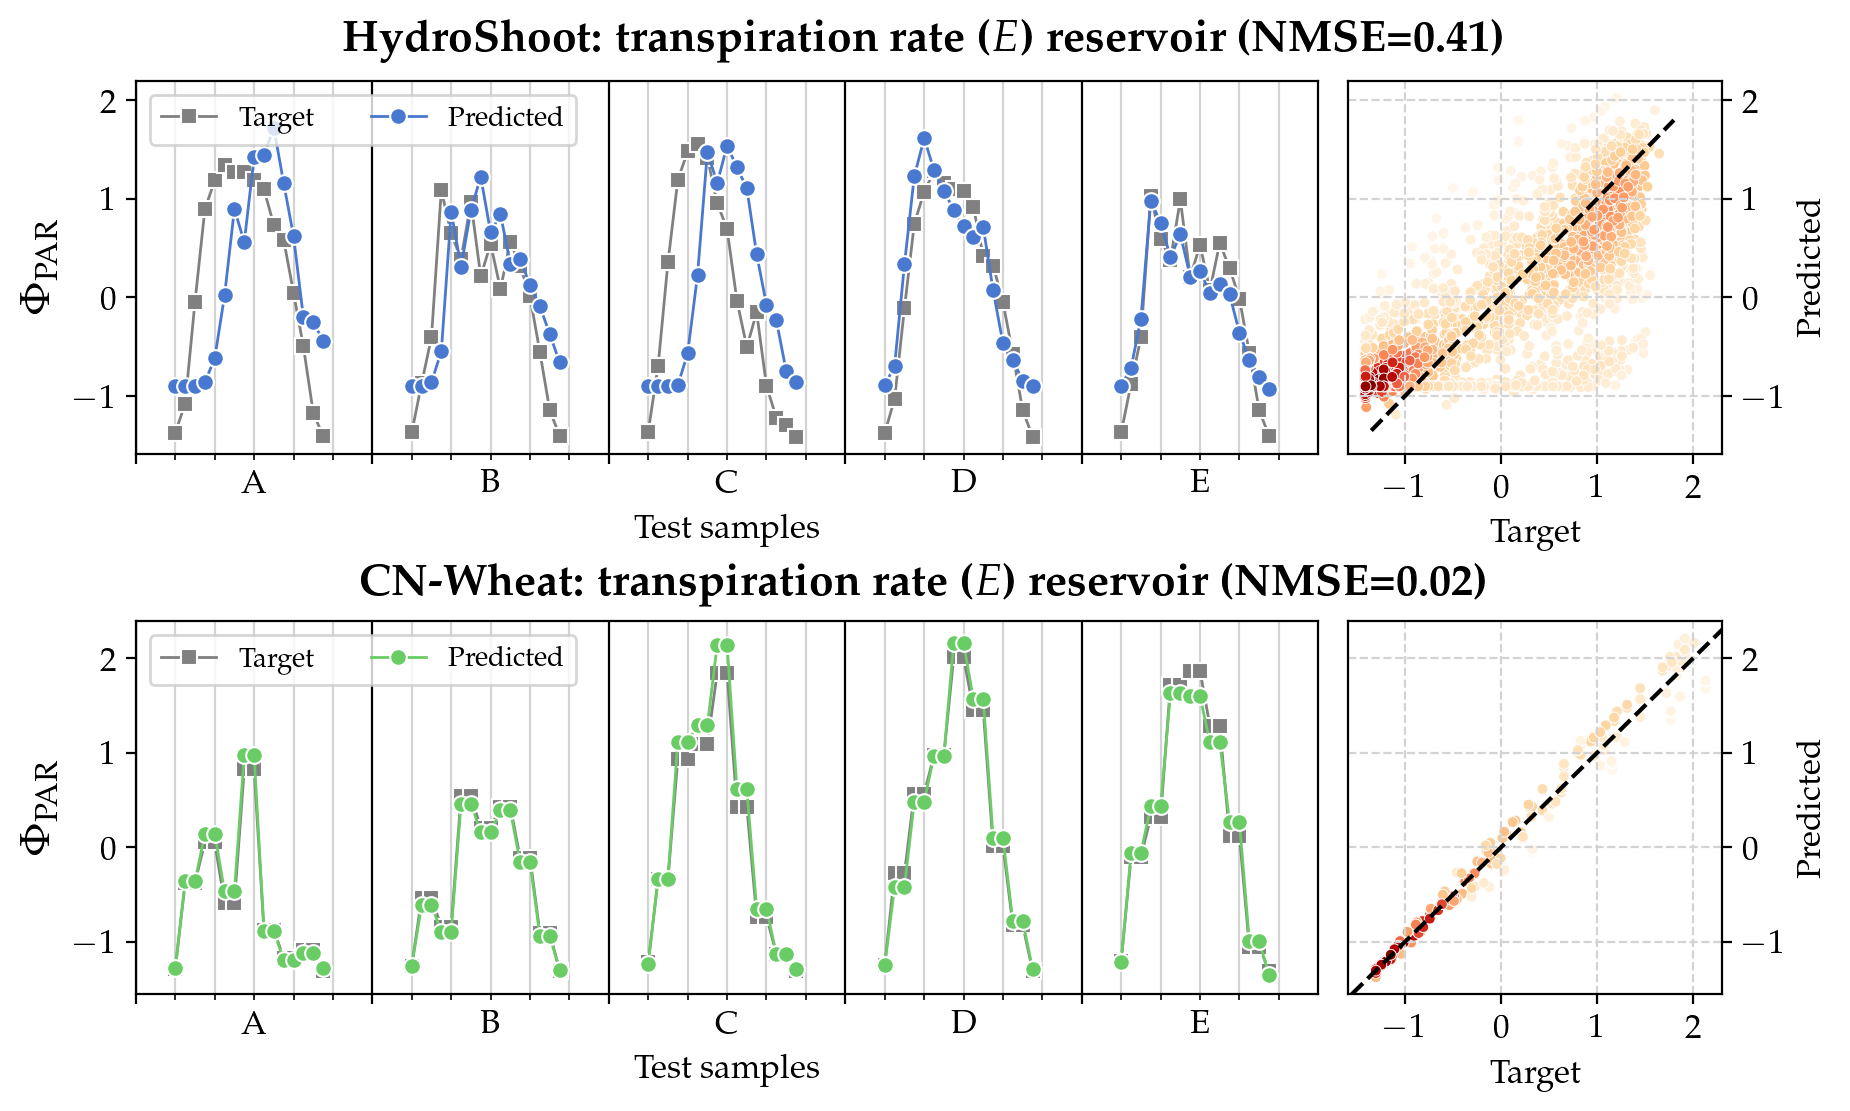
\includegraphics[width=\linewidth,keepaspectratio]{img/regression_res_prediction__output__custom__PARa__state__Tr.png}
        \caption{Time series prediction of absorbed PAR.}
    	\label{fig:predictions-phys}
	\end{subfigure}
	\caption[Time series prediction of input PAR and absorbed PAR using transpiration rate ($E$).]
	        {Time series prediction of input PAR and absorbed PAR using transpiration rate ($E$).
	         The left plot shows time series prediction for five random samples from the test set (see \mbox{Section \ref{sec:train-test-split}}),
	         the right shows the correlation between the target and predicted values. Darker colors indicate a greater density of points.}
	\label{fig:predictions-input-phys}
\end{figure}

% 	- *Caption:*
% 		- Left plots: time series prediction for five random samples from the test set (see Section 6.4).
% 		- Right plots: Correlation between target values and predicted values.
% 			- Points above the dashed line are overpredictions, points under it are underpredictions.
